\documentclass{article}
\usepackage[margin=3.5cm]{geometry}
\usepackage[latin1]{inputenc}
\usepackage[T1]{fontenc}
\usepackage[english]{babel}
\usepackage{float}
\usepackage{graphicx}
\usepackage{amsmath}
\usepackage{amsthm}
\usepackage{mathtools}
\usepackage{listings}
\usepackage{qtree}
\usepackage{caption}
\usepackage{subcaption}
\usepackage{amssymb}
\newtheorem{thm}{Theorem}[section]
\theoremstyle{definition}
\newtheorem{defi}{Definition}[section]
\newtheorem{nota}{Notation}[section]
\theoremstyle{remark}
\newtheorem{rem}{Remark}[section]
\theoremstyle{proposition}
\newtheorem{prop}{Proposition}[section]
\newtheorem{lem}{Lemma}[section]
\newtheorem{ex}{Example}[section]
\usepackage{hyperref}

\begin{document}
	\title{A deeper dive into \textit{A novel statistical approach to analyze image classification} by Juntong Chen, Sophie Langer and Johannes Schmidt-Hieber}
	\author{Yanis \textsc{BOSCH}}
	\maketitle
	\newpage
	\tableofcontents
	\newpage
	\section{Introduction}
        \section{Framework and definitions}
            \subsection{Images and deformations}
            For any integers $i,j \in \mathbb{Z}$ we define:
            \[
                I_{j,l} := \left[ \frac{j-1}{d},\frac{j}{d} \right[ \times \left[ \frac{l-1}{d},\frac{l}{d} \right[
            \]
            a pixel of size $\frac{1}{d}\times \frac{1}{d}$.

            IMAGE DEFINITION

            DEFORMATION DEFINITION

            CONDITIONS ON DEFORMATIONS

            EXAMPLES OF POSSIBLE DEFORMATIONS
        \section{Classification via inverse mappings and image alignment}

        APPROX OF INVERSE TRANSFORMATION SET

        DEFINITION OF FIRST CLASSIFIER

        ASSUMPTIONS ON DEFORMATION

        MISCLASSIFICATION BOUNDS 

        SAME AGAIN FOR CLASSIFICATION VIA IMAGE ALIGNMENT
        
        \section{CNN}
        \subsection{CNN Definition}

        STRUCTURE OF THE CNN

        COUNTEREXAMPLE TO SHOW IMPORTANCE OF SEPARATION QUANTITY
        
        \subsection{Performance metrics}

        EXISTENCE OF OPTIMAL CNN

        CONSTRUCTABLE CNN + UPPER BOUND ON ITS MISCLASSIFICATION
        
        \section{Code}
            In the following section our work is based by the code provided by Sophie Langer in \cite{Image-deformation-model}. In particular the code for generating data with a single template, visualizing data and the image classification algorithms were carried over to our work.

            

            \subsection{Empirical distance}

            In the previous sections we used separation quantities between two template functions in order to introduce upper bounds on misclassifications. However, in practice, we do not know these template functions. When computing the average intensity of these templates over the individual pixels, a lot of information is lost. There exist many functions that would yield the same image after computing the integrals over each pixel.

            As an interesting note, all information about Lipchitz continuity of our template functions is also lost. However, in order to confirm the computed upper bounds through computation, one could still define template functions, generate a dataset based on these, and apply our image classification algorithms.

            Thus, in order to get a better idea of the relationship between the defined separation quantity $D := D(f_0,f_1) \vee D(f_1,f_0)$ defined in INSERT REF HERE and the performance of our classification algorithms, we will define an empirical substitute for this distance, i.e. a quantity that depends only the images used for training. Suppose that our data is of the form $(X_i,k_i)$ for $i\in \{1,...,n\}$ where $n\in\mathbb{N}$. $X_i$ denotes the $i^{th}$ image, and $k_i$ denotes its label. We let:
            \[
                K_0 := \left\{ X_i : k_i = 0 \right\} \quad \text{and} \quad K_1 := \left\{ X_i : k_i = 1 \right\}
            \]
            and suppose that these sets are both non empty. Then we define the empirical distance separating our two classes as:
            \[
                \tilde{D}:=\min_{X_0 \in K_0, X_1 \in K_1} \tilde{D}(X_0,X_1)
            \]
            where:
            \[
                \tilde{D}(X_0,X_1) := \inf_{A\in\mathcal{A},A' \in \mathcal{A}^{-1},a,s,s'\in \mathbb{R}} \| a X_0 \circ A' \circ A(\cdot + s, \cdot + s') - X_1 \| _{L^2 (\mathbb{R}^2)} \frac{1}{ \| X_1 \| _{L^2 (\mathbb{R}^2)} }
            \]
            with $\mathcal{A}$ defined as in INSERT REF HERE. Here we first minimize over all possible inverse transforms in order to iterate over all potential template functions. Note that these are not continuous functions as one would expect from a template function, as these have constant values over each pixel.S 
            
            TO CHECK We also expect this quantity to be larger than the separation quantity $D$, as we are only minimizing over a subset of all possible transformed images. TO CHECK

            In practice this still remains computationally very expensive. Moreover, our set of transforms will most likely not be discrete. Thus, in practice we sample a set amount of inverse transforms and apply them to our templates. We repeat the same with regular transforms applied to all our newly computed images.
            
            However, this is a stochastic process, and the result seem to be quite variable. In practice, we sampled ten inverse transforms and ten transforms, yielding 100 images. This was computationally already quite expensive, yet our results still varied very strongly, as shown in these plots:
            
            \begin{figure} [H]
                \centering
                \begin{subfigure}{.5\textwidth}
                      \centering
                      \includegraphics[width=0.9\linewidth]{Images/Emp_dist_1vs9_1temp_1.png}
                      %\caption{A subfigure}
                      %\label{fig:sub1}
                \end{subfigure}%
                \begin{subfigure}{.5\textwidth}
                      \centering
                      \includegraphics[width=0.9\linewidth]{Images/Emp_dist_1vs9_1temp_2.png}
                      %\caption{A subfigure}
                      %\label{fig:sub2}
                \end{subfigure}
                \caption{Computed empirical distances between $1$ and $9$ with $1$ template per class}
                \label{1vs9_1t}
            \end{figure}


            Moreover, one would expect the distance between the digits $1$ and $7$ to be very small, as one can obtain very similar images by rotating one digit to match the other. However, for this to be reflected in our empirical distance, one would need to sample the right transforms to achieve this rotation. Thus we sometimes obtain a much larger empirical distance than expected between these digits. 

            \begin{figure}[H]
                \centering
                \begin{subfigure}{.5\textwidth}
                      \centering
                      \includegraphics[width=0.9\linewidth]{Images/Emp_dist_1vs7_1temp_1.png}
                      %\caption{A subfigure}
                      %\label{fig:sub1}
                \end{subfigure}%
                \begin{subfigure}{.5\textwidth}
                      \centering
                      \includegraphics[width=0.9\linewidth]{Images/Emp_dist_1vs7_1temp_2.png}
                      %\caption{A subfigure}
                      %\label{fig:sub2}
                \end{subfigure}
                \caption{Computed empirical distances between $1$ and $7$ with $1$ template per class}
                %\label{fig:test}
            \end{figure}

            One can see here that the computed empirical distance between $1$ and $7$ varies quite strongly. In one case we obtain a distance of about $0.31$ and in the other case about $0.375$. This however still serves as a rough estimate, as we can see that in the general the distance between $1$ and $9$ is higher than the distance between $1$ and $7$, as expected.

            \subsection{Multiple template functions}

            One of the main limitations of the models discussed before is that they are based on the assumption that each image is generated by one of two template function, one for each class. In practice this seems unlikely. For example, one could draw the digits $1$ and $7$ in multiple ways, as shown here:

            \begin{figure}[H]
                \centering
                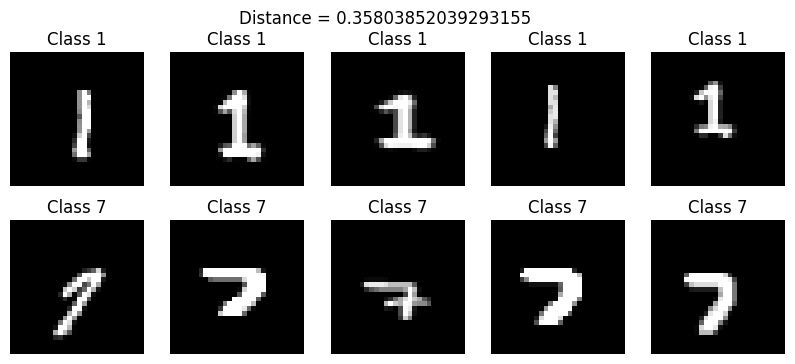
\includegraphics[width=0.9\linewidth]{Images/1vs7_vis_4temp}
                \caption{Generated images for the digits $1$ and $7$ using $4$ templates for each}
                \label{1vs9_vis_4t}
            \end{figure}

            Thus it would make sense to study how much this impacts the performance of our classifiers. Due to time constraints, this will done computationally in section~\ref{code_results}. 
            
            Let us start by denoting by $F_0$ the set of all template functions for class $0$, and $F_1$ the set for the class $1$. The definition of the separation quantity $D$ can be extended to this case as follows:
            
            \[
                D := \min_{f_0 \in F_0,f_1 \in F_1} D(f_0,f_1) \vee D(f_1,f_0)
            \]

            The definition given for $\tilde{D}$ can be carried over without modification to the case where we use multiple template functions.
            Given that we are now minimizing over all pairs of template functions, we expect these separation quantities to be smaller or equal to their single template counterparts. We can verify this by implementing a function that generates samples from two chosen digits using more than one template function per digit.This yielded the following results:
            
            \begin{figure}[H]
                \centering
                \begin{subfigure}{.5\textwidth}
                      \centering
                      \includegraphics[width=0.9\linewidth]{Images/Emp_dist_1vs7_4temp_1.png}
                      %\caption{A subfigure}
                      %\label{fig:sub1}
                \end{subfigure}%
                \begin{subfigure}{.5\textwidth}
                      \centering
                      \includegraphics[width=0.9\linewidth]{Images/Emp_dist_1vs7_4temp_2.png}
                      %\caption{A subfigure}
                      %\label{fig:sub2}
                \end{subfigure}
                \caption{Computed empirical distances between $1$ and $7$ with $1$ vs $4$ templates per class}
                %\label{fig:test}
            \end{figure}

            While we observe the same high variability in the obtained values, we can notice that they are overall smaller than those obtained in figure~\ref{1vs9_1t}. This aligns with our expectation. In particular, for the digits $1$ and $7$, as we pick more templates, we are likely to pick templates where the way we write $1$ and $7$ resemble each other (for example we can more likely pick a $7$ without the horizontal line, see figure~\ref{1vs9_vis_4t}).
            
            Moreover we can note the following:
            \begin{lem}
                Let $X_i$ and $X_j$ be two distinct images obtained from the same template function $f$. Thus, $\exists A_i,A_j \in \mathcal{A}$ such that:
                \[
                    \begin{array}{c}
                        X_i = f \circ A_i \\
                        X_j = f \circ A_j
                    \end{array}
                \]
                Then:
                \[
                    \tilde{D} (X_i,X_j) = \tilde{D} (X_j,X_i) = 0
                \]
            \end{lem}
            \begin{proof}
                By assumption we know that $\exists A_i,A_j \in \mathcal{A}$ such that $X_i = f \circ A_i$ and $X_j = f \circ A_j$. Thus $\exists A_i^{-1},A_j^{-1} \in \mathcal{A}$ such that:
                \[
                    \begin{array}{c}
                        X_i \circ A_i^{-1} = f \\
                        X_j \circ A_j^{-1} = f
                    \end{array}
                \]
                Thus:
                \begin{align*} 
                    \tilde{D}(X_i,X_j) &= \inf_{A\in\mathcal{A},A' \in \mathcal{A}^{-1},a,s,s'\in \mathbb{R}} \| a X_i \circ A' \circ A(\cdot + s, \cdot + s') - X_j \| _{L^2 (\mathbb{R}^2)} \frac{1}{ \| X_j \| _{L^2 (\mathbb{R}^2)} } \\ 
                    & \leq \| X_i \circ A_i^{-1} \circ A_j - X_j \| _{L^2 (\mathbb{R}^2)} \frac{1}{ \| X_j \| _{L^2 (\mathbb{R}^2)} } \\
                    & \leq \| X_j - X_j \| _{L^2 (\mathbb{R}^2)} \frac{1}{ \| X_j \| _{L^2 (\mathbb{R}^2)} } \\
                    & = 0
                \end{align*}
                The same proof works for $\tilde{D}(X_j,X_i)$.
            \end{proof}

            I.e., for any two images that can be obtained by the same template function, we expect the distance between them to be $0$. This means that $\tilde{D}$ is not a distance, as $\tilde{D}(X,Y) = 0 \nRightarrow X = Y$. We also expect the images to be clustered with respect to this separation quantity, with each template giving one point-like cluster.
    
            Given this, using measures that define distances between clusters is uninteresting, which is why simply minimize the distance over all possible pairs instead of using a measure like INSERT MEASURES HERE.

            \subsection{Results and comments on these}
            \label{code_results}

            We implemented the procedure by image alignment, and three neural networks with the following structures:
            \[
                \begin{array}{|c|c|c|c|}
                    \hline
                    & \text{CNN}1 & \text{CNN}2 & \text{CNN}3 \\
                    \hline
                    \# \text{convolutional layers} & 1 & 3 & 3 \\
                    \text{filter sizes} & 32\times32 & 32\times32, 64\times64, 128\times128 & 32\times32, 64\times64, 128\times128 \\
                    \text{max-pooling layer patch size} & 2 \times 2 & 2\times2 & 2\times2 \\
                    \# \text{fully connected layers} & 1 & 1 & 2 \\
                    \# \text{neurons per layer} & 128 & 128 & 256,128 \\
                    \hline
                \end{array}
            \]

            This yielded the following results:

            \begin{figure}[H]
                \centering
                \begin{subfigure}{.5\textwidth}
                      \centering
                      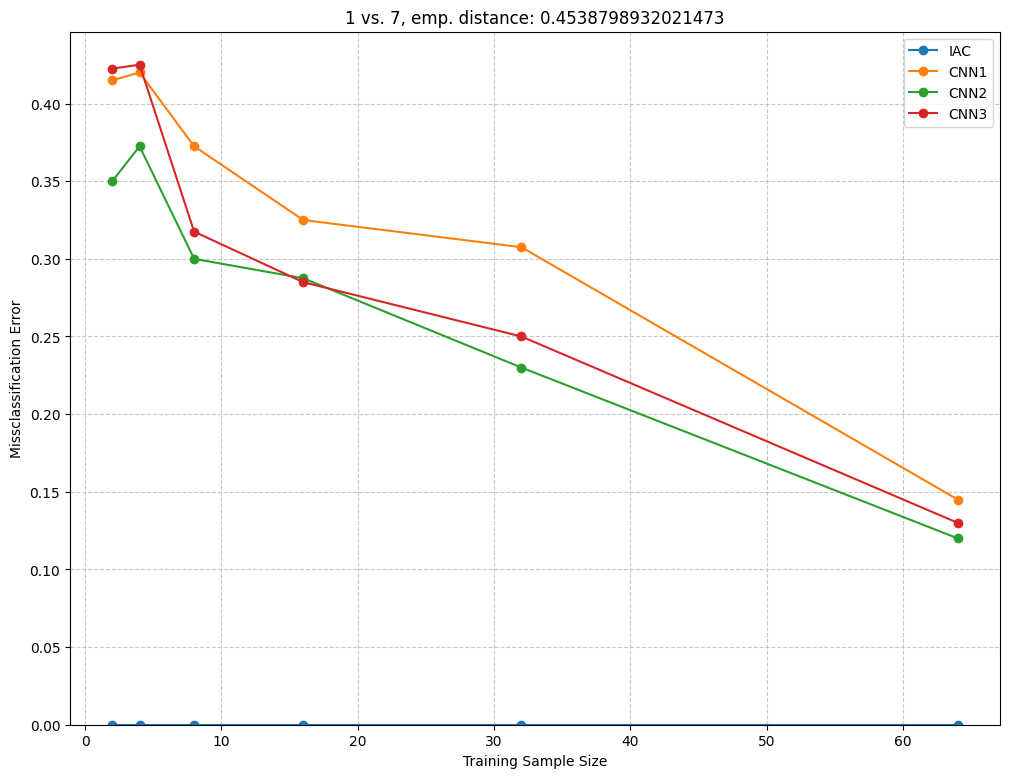
\includegraphics[width=0.9\linewidth]{Images/1vs7_1temp.png}
                      %\caption{A subfigure}
                      %\label{fig:sub1}
                \end{subfigure}%
                \begin{subfigure}{.5\textwidth}
                      \centering
                      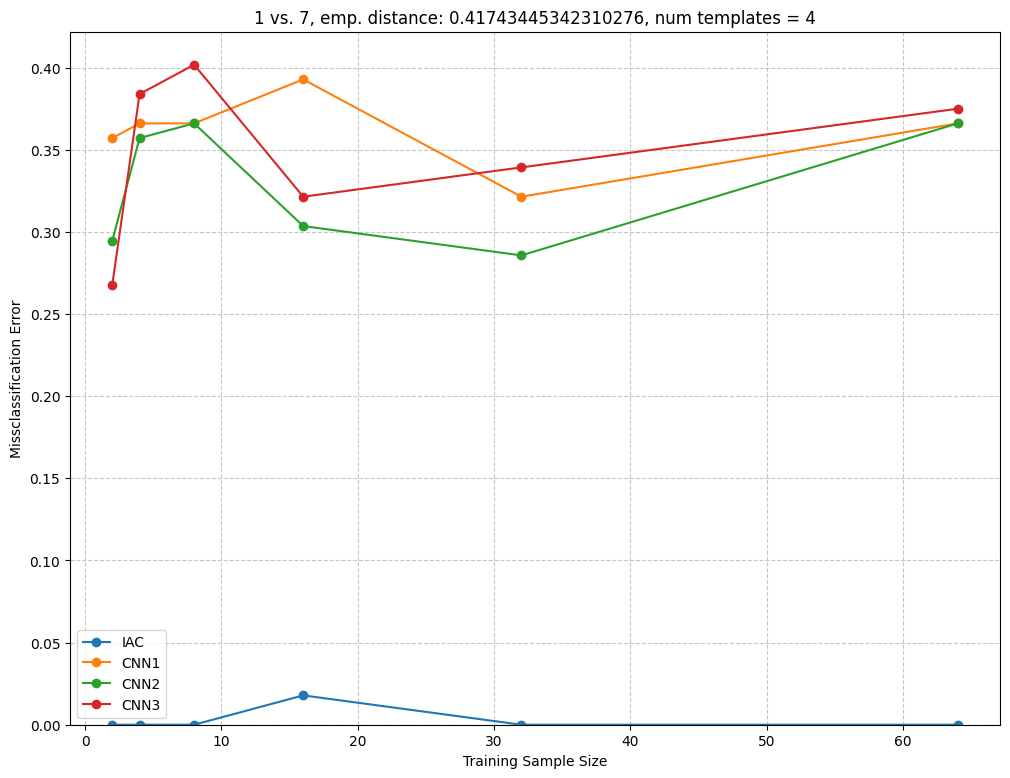
\includegraphics[width=0.95\linewidth]{Images/1vs7_4temp.png}
                      %\caption{A subfigure}
                      %\label{fig:sub2}
                \end{subfigure}
                \caption{Misclassification error for $1$ vs $7$}
                %\label{fig:test}
            \end{figure}
            \begin{figure}[H]
                \centering
                \begin{subfigure}{.5\textwidth}
                      \centering
                      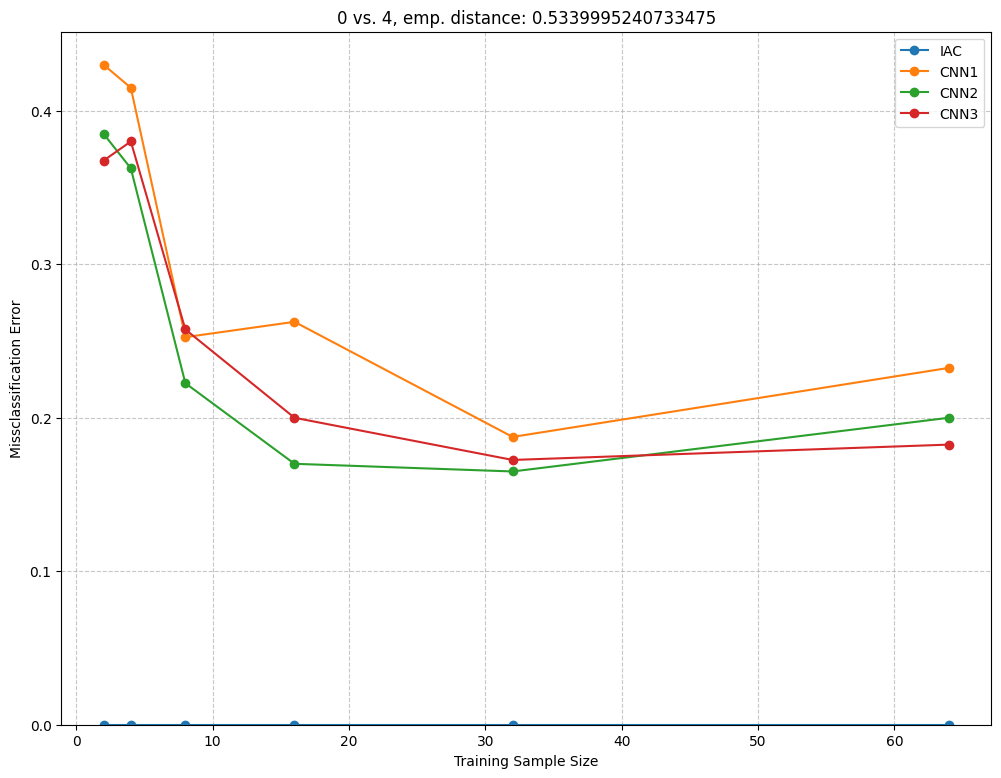
\includegraphics[width=0.9\linewidth]{Images/0vs4_1temp.png}
                      %\caption{A subfigure}
                      %\label{fig:sub1}
                \end{subfigure}%
                \begin{subfigure}{.5\textwidth}
                      \centering
                      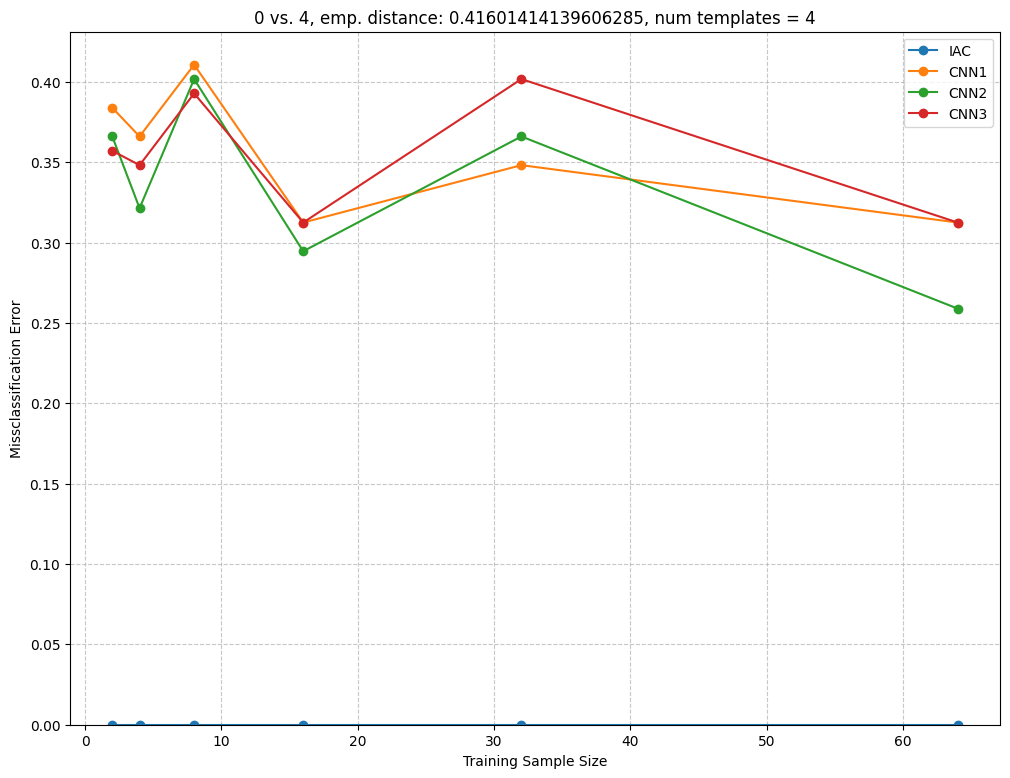
\includegraphics[width=0.95\linewidth]{Images/0vs4_4temp.png}
                      %\caption{A subfigure}
                      %\label{fig:sub2}
                \end{subfigure}
                \caption{Misclassification error for $0$ vs $4$}
                %\label{fig:test}
            \end{figure}

            The first things that catches the attention upon seeing these graphs is the fact that

            We can notice is that the empirical distance seems to correlate quite nicely with the performance of our algorithms. When we use $1$ template we obtain empirical distances of $0.518$ and $0.511$ respectively, yielding misclassification rates of $25\%$ and $20\%$ respectively. Note that here, contrary to our intuition, the distance between $1$ and $7$ is quite similar to that between $0$ and $4$. This most likely means that we picked templates for $1$ and $7$ that differ sufficiently. This similarity quickly subsides when picking $4$ templates, as we have more chances of obtaining similar templates for these two digits.
            
            THE CIA ALWAYS WORKS VERY WELL: EXTREMELY SPECIFIC CASE WHERE IT IS IMPOSSIBLE TO DEFORM ONE CLASS INTO THE OTHER 

        \section{Potential additions}

        DICE NUMBER RECOGNITION

        IN DEPTH ANALYSIS OF THE EMPIRICAL DISTANCE

        CHECK MORE IN DETAIL IF WE CAN REPLACE DISTANCE WITH MULTI TEMPLATE VERSION

        WE DONT HAVE TEMPLATE FUNCTION, BUT WE COULD DESIGN THE TEMPLATE WITH THE LOWEST POSSIBLE LIPSCHITZ CONSTANT TO LOWER THE BOUNDS (WE EXPECT A MINIMAL CONSTANT AS THE FUNCTION WILL HAVE A CERTAIN AVERAGE VALUE TO REACH ON EACH PIXEL, LEADING TO CERTAIN "MINIMAL" FLUCTUATIONS
        
        \cite{arXiv:2206.02151v2}
        \cite{Image-deformation-model}
\bibliographystyle{abbrv}
\bibliography{sample}
\end{document}

